\section{Test Description and Success Criteria}
This test is located in \texttt{SimCode/dynamics/HingedRigidBodies/UnitTest/\newline
test\_hingedRigidBodyStateEffector.py}. In this integrated test there are two hinged rigid bodies connected to the spacecraft hub.  Depending on the scenario, there are different success criteria. These are outlined in the following subsections:
\subsection{Gravity and no damping scenario}
In this test the simulation is placed into orbit around Earth with point gravity and has no damping in the hinged rigid bodies. The following parameters are being tested. 
\begin{itemize}
	\item Conservation of orbital angular momentum
	\item Conservation of orbital energy
	\item Conservation of rotational angular momentum
	\item Conservation of rotational energy
	\item Achieving the expected final attitude
\end{itemize}

\subsection{No gravity and no damping scenario}
In this test, the spacecraft is placed in free space (no gravity) and has no damping in the hinged rigid bodies. The following parameters describe the success criteria.
\begin{itemize}
\item Conservation of orbital angular momentum
\item Conservation of orbital energy
\item Conservation of rotational angular momentum
\item Conservation of rotational energy
\item Achieving the expected final attitude (same final attitude as the Gravity with no damping scenario)
\item Achieving the expected final position
\item Conservation of velocity of center of mass
\end{itemize}

\subsection{No gravity with damping scenario}
In this test, the spacecraft is placed in free space (no gravity) and has damping in the hinged rigid bodies. The following parameters describe the success criteria.
\begin{itemize}
\item Conservation of orbital angular momentum
\item Conservation of orbital energy
\item Conservation of rotational angular momentum
\item Conservation of velocity of center of mass
\end{itemize}

\subsection{Steady State Deflection Verification Scenario}

The BOE calculation for the steady state deflection can be seen in Fig.~\ref{fig:BOEThetaSS}. As it can be seen the resulting steady state deflection does not have a closed form solution so a root solving function must be used to converge on the solution. A Newton-Raphson method was chosen and the success criteria for this test is whether Basilisk gives the same results as this BOE calculation within a certain tolerance. The spacecraft has a constant force applied through the whole simulation with the hinged rigid bodies initially undeflected and they have damping. The force is always applied through the center of mass of the spacecraft and results in no rotation of the spacecraft. 

\begin{figure}[htbp]
	\centerline{
		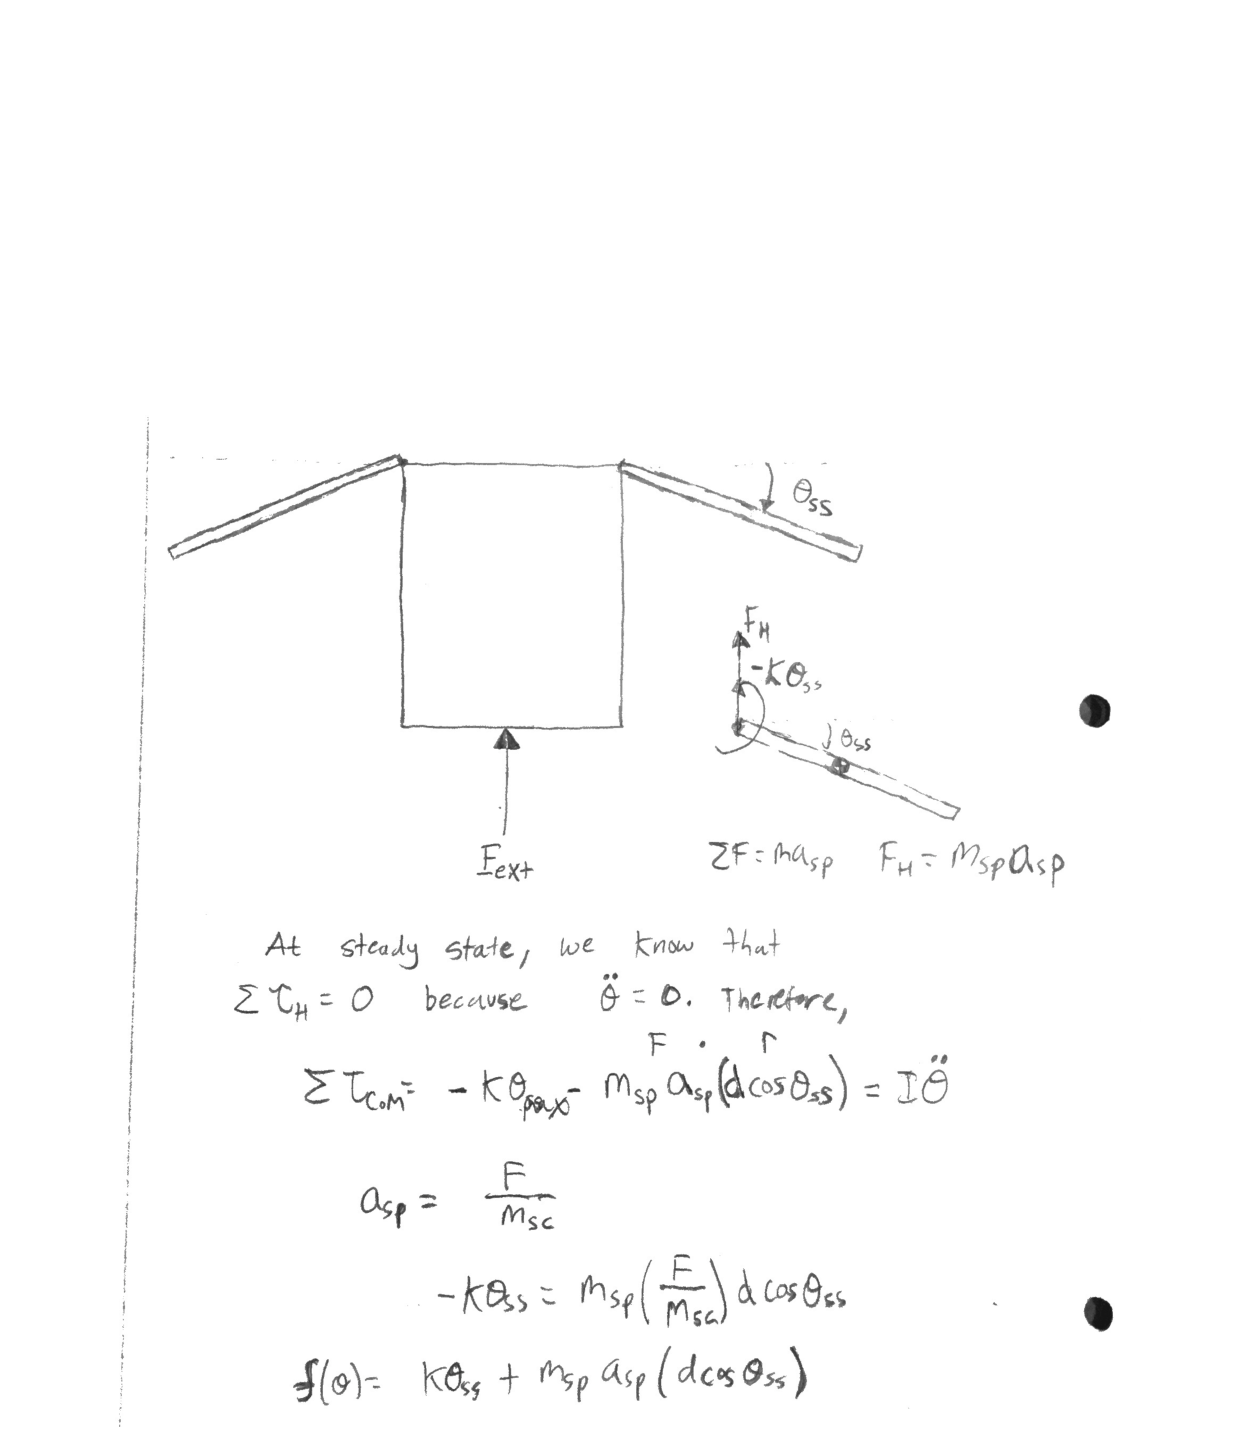
\includegraphics[width=0.8\textwidth]{Figures/BOEThetaSS}}
	\caption{Steady State Deflection BOE Calculation}
	\label{fig:BOEThetaSS}
\end{figure}

\subsection{Frequency and Amplitude Verification Scenario}

The BOE calculation for the frequency of oscillation of flexing hinged rigid bodies when a constant force is being applied to the spacecraft is done by making simplifications to the flexing equation seen in the Model Description Section. The following assumptions are made to simplify the equations:

\begin{enumerate}
	\item The force is being directed through the center of mass of the spacecraft, along the $\hat{\bm b}_2$ direction
	\item The panels are initially undeflected and they are symmetric therefore the body will not rotate
	\item Rotation is no longer apart of the equations so the translation and solar panel equations are the only equations needed
	\item $\hat{\bm s}_{i,3}$ is assumed to be equal to $\hat{\bm h}_{i,3}$ in the equations of motion \label{item:4}
	\item No external torque is being applied directly to the hinged rigid bodies
	\item Non-linear terms are neglected \label{item:5}
\end{enumerate}
Using the third assumption from above, the rotational motion is taken out of the equations of motion:

\begin{equation}
m_{\text{sc}} \ddot{\bm r}_{B/N}+\sum_{i}^{N}m_{\text{sp}_i} d_i  \bm{\hat{s}}_{i,3}\ddot{\theta}_i = \bm F_{\textnormal{ext}} -\sum_{i}^{N}m_{\text{sp}_i}d_i\dot{\theta}_i^2 \bm{\hat{s}}_{i,1}
\label{eq:Rbddot6}
\end{equation}

\begin{equation}
m_{\text{sp}_i} d_i \hat{\bm s}_{i,3}^{T} \ddot{\bm r}_{B/N} 
+ \left( I_{s_{i,2}} + m_{\text{sp}_i} d_i^{2} \right) \ddot \theta_i 
= - k_i \theta_i - c_i \dot\theta_i + \hat{\bm s}_{i,2}^T \bm \tau_{\text{ext},H_i}  
\label{eq:solar_panel_final9}
\end{equation}
Next, assumptions \ref{item:4}-\ref{item:5} are applied:
\begin{equation}
m_{\text{sc}} \ddot{\bm r}_{B/N}+\sum_{i}^{N}m_{\text{sp}_i} d_i  \bm{\hat{h}}_{i,3}\ddot{\theta}_i = \bm F_{\textnormal{ext}}
\label{eq:Rbddot7}
\end{equation}

\begin{equation}
m_{\text{sp}_i} d_i \hat{\bm h}_{i,3}^{T} \ddot{\bm r}_{B/N} 
+ \left( I_{s_{i,2}} + m_{\text{sp}_i} d_i^{2} \right) \ddot \theta_i 
= - k_i \theta_i - c_i \dot\theta_i  
\label{eq:solar_panel_final10}
\end{equation}
Finally, knowing that the force is being directed along the $\hat{\bm b}_2$ axis and that the spacecraft will not rotate, the equations simplify to:
\begin{equation}
m_{\text{sc}} \ddot{y}_{B/N}+\sum_{i}^{N}m_{\text{sp}_i} d_i \ddot{\theta}_i = F_{y}
\label{eq:Rbddot9}
\end{equation}

\begin{equation}
m_{\text{sp}_i} d_i \ddot{y}_{B/N} 
+ \left( I_{s_{i,2}} + m_{\text{sp}_i} d_i^{2} \right) \ddot \theta_i 
= - k_i \theta_i - c_i \dot\theta_i  
\label{eq:solar_panel_final12}
\end{equation}
Converting these equations to state space:
\begin{multline}
\begin{bmatrix}
1 & 0 & 0 & 0 & 0 & 0\\
0 & m_{\text{sc}} & 0 & m_{\text{sp}_1} d_1 & 0 & m_{\text{sp}_2} d_2 \\
0 & 0 & 1 & 0 & 0 & 0\\
0 & m_{\text{sp}_1} d_1 & 0 &  I_{s_{1,2}} + m_{\text{sp}_1} d_1^{2} & 0 & 0 \\
0 & 0 & 0 & 0 & 1 & 0\\
0 & m_{\text{sp}_2} d_2 & 0 & 0 & 0 & I_{s_{2,2}} + m_{\text{sp}_2} d_2^{2} \\
\end{bmatrix}
\begin{bmatrix}
\dot{y}_{B/N} \\
\ddot{y}_{B/N} \\
\dot \theta_1 \\
\ddot \theta_1 \\
\dot \theta_2 \\
\ddot \theta_2 \\
\end{bmatrix}
\\
=\begin{bmatrix}
0 & 1 & 0 & 0 & 0 & 0\\
0 & 0 & 0 & 0 & 0 & 0\\
0 & 0 & 0 & 1 & 0 & 0\\
0 & 0 & -k_1 & -c_1 & 0 & 0\\
0 & 0 & 0 & 0 & 0 & 1\\
0 & 0 & 0 & 0 & -k_2 & -c_2\\
\end{bmatrix}
\begin{bmatrix}
{y}_{B/N} \\
\dot{y}_{B/N} \\
\theta_1 \\
\dot \theta_1 \\
\theta_2 \\
\dot \theta_2 \\
\end{bmatrix}
+ \begin{bmatrix}
0 \\
F_y \\
0 \\
0 \\
0 \\
0 \\
\end{bmatrix}
\label{eq:solar_panel_final13}
\end{multline}
Written in a more compact form:
\begin{equation}
[M] \dot{\bm X} = [A] \bm X + \bm F
\end{equation}
The equivalent dynamics matrix for this coupled system is:
\begin{equation}
[\tilde{A}] = [M][A]
\end{equation}

Finding the eigenvalues of $[\tilde{A}]$ will describe the coupled natural frequencies of the combined system. The integrated test for this scenario ensures that the analytical coupled frequency of oscillation matches the frequency obtained from the simulation. 

The next BOE calculation that is needed is to find the maximum deflection while the force is being applied and when the force is not being applied (with the assumption that there is no damping). When the force is being applied the following max deflection can be seen in the following equation:

\begin{equation}
\theta_{\textnormal{max}} = 2 \theta_{\textnormal{SS}}
\end{equation}
which uses the definition of $\theta_{\textnormal{SS}}$ from Fig.~\ref{fig:BOEThetaSS}. 

Finally, the maximum deflection when the force is not being applied uses approximate energy techniques seen in the following equations:

\begin{equation}
E_0 = \frac{1}{2} I_{\textnormal{sp}} \dot{\theta}(t_{\textnormal{off}})^2 + \frac{1}{2} m_{\textnormal{sp}} \Big[d \dot{\theta}(t_{\textnormal{off}})\Big]^2 + \frac{1}{2} k \theta(t_{\textnormal{off}})^2
\end{equation}

$E_0$ is the energy when force is turned off and time: $t_{\textnormal{off}}$. Next the max deflection can be approximated by using the following equation: 

\begin{equation}
\theta_{\textnormal{max}} = \sqrt{\frac{2 E_0}{k}}
\end{equation}

Again, just like the frequency BOE calculation, this is an approximation and neglects the energy stored in the spacecraft hub that a portion will be transfered to the oscillations. The test results for both the frequency and this maximum deflection reflects this approximation in the tolerances. 

\subsection{Lagrangian vs Basilisk Scenario}

In this scenario the equations of motion for a planar simulation of a spacecraft hub and two hinged rigid bodies using Lagrangian mechanics was developed using Mathematica. The mathematica script can be seen in the support folder in the following file name: PlanarFlexibleDynamicsDerivation. This simulation is ran independently in the integrated test and the results are compared vs Basilisk results. A force and torque is applied for a certain amount of time, then turned off. Then another pulse of a force and torque is applied and turn off and the simulation runs for another few seconds.



